\documentclass[11pt]{article}
\usepackage[a4paper,margin=1in]{geometry}
\usepackage{amsmath,amssymb}
\usepackage{graphicx}
\usepackage{booktabs}
\usepackage{caption}
\usepackage{subcaption}
\usepackage{float}
\usepackage{xcolor}
\usepackage[hidelinks]{hyperref}
\usepackage{enumitem}
\usepackage{parskip}
\title{\textbf{Digital Image Processing --- Assignment 2}\\[0.3em]\large Problem 3: Homomorphic Filtering: Illumination and Reflectance}
\author{Ujjwal Gupta}
\date{\today}
\begin{document}
\maketitle
\tableofcontents
\vspace{1em}

\section{Introduction / Problem Statement}

Problem 3 of the assignment (worth 10 of the 100 total marks) asks for a treatment of
\emph{homomorphic filtering} applied to an unevenly lit photograph --- the specification
calls for ``an unevenly lit photograph (deep shadow and bright region in one frame -- a
doorway, a backlit face, an image with strong vignetting)''. The problem is split into
two parts:

\begin{itemize}[leftmargin=1.5em]
  \item \textbf{3.1 The multiplicative model (4 pts).} State the model
  $I(x,y) = L(x,y)R(x,y)$, derive why taking the log converts this into an additive
  problem that a linear frequency-domain filter can act on, and explain precisely why
  the log must be taken \emph{before} the Fourier transform rather than after.
  \item \textbf{3.2 Implement and tune (6 pts).} Implement the homomorphic
  high-frequency-emphasis filter
  $H(u,v) = (\gamma_H-\gamma_L)\left[1-e^{-cD^2(u,v)/D_0^2}\right]+\gamma_L$ applied to
  $\log I$, sweep its parameters to identify settings that flatten illumination while
  preserving local contrast versus settings that produce visible halos, and compare the
  result against plain global histogram equalisation using a local-contrast metric.
\end{itemize}

This problem matters in digital image processing because it is the canonical example of
a situation where a \emph{nonlinear} pre-transform (the logarithm) is required to make a
\emph{linear} tool (frequency-domain filtering) applicable to a physically multiplicative
process. Ordinary photographs of scenes with strong, uneven lighting --- a tunnel with a
light source at one end, a backlit doorway, a face lit from one side --- are not well
described by an additive noise/signal model; they are far better modelled as the product
of a slowly varying illumination field and a rapidly varying surface reflectance. Simple
global contrast operations such as histogram equalisation have no notion of this
underlying physical separation and can therefore fail badly (as quantified in Section~5),
whereas homomorphic filtering exploits the structure of the model directly.

\section{Theoretical Background}

\subsection{The multiplicative illumination--reflectance model}

An image intensity $I(x,y)$ formed by a camera observing a diffusely reflecting scene
under incident illumination is well modelled as the product
\begin{equation}
  I(x,y) = L(x,y)\,R(x,y),
  \label{eq:model}
\end{equation}
where $L(x,y) \ge 0$ is the \emph{illumination} component -- the amount of light
striking the scene at each point, which is physically constrained to vary
\emph{slowly} in space (it is governed by large-scale geometry: distance to the light
source, shading, vignetting) -- and $R(x,y) \in [0,1]$ is the \emph{reflectance}
component -- the fraction of incident light reflected by the surface at each point,
which varies \emph{rapidly}, carrying the fine detail, edges and texture of the scene
(material boundaries, surface markings). Crucially, $L$ dominates the \emph{low}
spatial frequencies of $I$ and $R$ dominates the \emph{high} spatial frequencies.

\subsection{Why the logarithm converts the problem to an additive one}

A linear, shift-invariant frequency-domain filter can only act on a signal by
reweighting the Fourier coefficients of an \emph{additive} decomposition of that
signal --- the Fourier transform is a linear operator, so it distributes over sums but
not over products:
\[
  \mathcal{F}\{a+b\} = \mathcal{F}\{a\}+\mathcal{F}\{b\}, \qquad
  \mathcal{F}\{a\cdot b\} = \mathcal{F}\{a\}\ast\mathcal{F}\{b\} \ \ (\text{convolution, not a simple product of spectra}).
\]
Equation~\eqref{eq:model} is a product, so no linear filter applied directly to $I$ can
separate $L$ from $R$ by frequency content -- multiplying two spatial signals
corresponds to \emph{convolving} their spectra, which mixes rather than separates
frequency content. Taking the natural logarithm of both sides of \eqref{eq:model},

\begin{align}
  \log I(x,y) &= \log\big(L(x,y)\,R(x,y)\big) \nonumber \\
              &= \log L(x,y) + \log R(x,y),
  \label{eq:logadd}
\end{align}

converts the multiplicative relationship into an \emph{additive} one. Because $L$ varies
slowly, $\log L$ is still concentrated in the low spatial frequencies; because $R$ carries
edges and texture, $\log R$ still contributes predominantly to the higher spatial
frequencies (the logarithm is a smooth, monotone, pointwise nonlinearity and does not
scramble this coarse frequency separation). A frequency-selective filter applied to
$\log I$ -- one that attenuates low frequencies (suppressing $\log L$) and boosts high
frequencies (emphasising $\log R$) -- can therefore separate the two \emph{additive}
terms by their frequency content in a way that was fundamentally impossible for the
original product $I = L R$. Exponentiating the filtered result afterward inverts the
logarithm and returns an image in which illumination has been flattened and reflectance
detail enhanced.

\subsection{Why the log must precede the Fourier transform, not follow it}

The homomorphic pipeline must be
\[
  \log I \ \xrightarrow{\ \mathcal{F}\ }\ \mathcal{F}\{\log I\} \ \xrightarrow{\times H(u,v)}\ H\cdot\mathcal{F}\{\log I\} \ \xrightarrow{\ \mathcal{F}^{-1}\ }\ \text{filtered } \log I \ \xrightarrow{\exp}\ \text{output},
\]
i.e.\ the logarithm must be taken on the \emph{spatial-domain image itself}, before any
Fourier transform. Two things go wrong if one instead tried to filter a
\emph{log-magnitude spectrum} $\log|\mathcal{F}\{I\}|$ -- the quantity ordinarily
computed only for \emph{display} purposes:

\begin{enumerate}[leftmargin=1.5em]
  \item \textbf{Phase is destroyed.} $\log|\mathcal{F}\{I\}|$ is a real, non-negative
  array built from the magnitude of the complex spectrum alone; all phase information
  has already been discarded by the $|\cdot|$ operation. As established for the
  phase/magnitude decomposition studied elsewhere in this assignment, phase carries the
  structural and positional information of an image, and no spatial-domain image can be
  reconstructed from a magnitude-only array -- there is simply nothing complex-valued
  left to invert.
  \item \textbf{$\log$ and $\mathcal{F}$ do not commute.} Even setting aside the phase
  problem, $\log|\mathcal{F}\{I\}| \ne |\mathcal{F}\{\log I\}|$ in general, because
  $\mathcal{F}$ is linear and $\log$ is not; filtering one quantity is not equivalent, even
  in principle, to filtering the other. This was verified numerically on the tunnel image
  used for this problem (Figure~\ref{fig:logorder}): $\log|\mathcal{F}\{I\}|$ and
  $\log|\mathcal{F}\{\log I\}|$, each normalised to zero mean/unit variance, have a
  correlation of only $0.669$ -- related in coarse shape (both are low-frequency-dominated,
  as any natural image's spectrum is), but clearly distinct quantities, not
  interchangeable.
\end{enumerate}

So the only correct order is: take the log of the real-valued spatial image first, then
Fourier-transform the result (preserving its full complex spectrum, magnitude and
phase), filter, inverse-transform, and finally exponentiate.

\subsection{The homomorphic high-frequency-emphasis filter}

The filter used is a Gaussian high-pass-like shape defined directly in the log domain:
\begin{equation}
  H(u,v) = (\gamma_H - \gamma_L)\left[1 - e^{-c\,D^2(u,v)/D_0^2}\right] + \gamma_L,
  \qquad \gamma_L < 1 < \gamma_H,
  \label{eq:homfilter}
\end{equation}
where $D(u,v)$ is the distance of frequency $(u,v)$ from the centre of the (zero-padded,
shifted) frequency plane, $D_0$ is a cutoff radius, and $c$ controls the sharpness of the
transition. At $D=0$ (DC, i.e.\ the low-frequency illumination term), the bracket
vanishes and $H(0,0) = \gamma_L < 1$, so the illumination component is \emph{attenuated}.
As $D \to \infty$ (high spatial frequencies, i.e.\ the reflectance/edge term), the
bracket tends to $1$ and $H \to \gamma_H > 1$, so reflectance detail is \emph{boosted}.
Because $\gamma_L<1<\gamma_H$, this single filter simultaneously compresses the dynamic
range contributed by illumination and sharpens the contribution of reflectance -- exactly
the desired homomorphic behaviour. $D_0$ controls where the transition between the two
regimes occurs: a small $D_0$ classifies more of the spectrum as ``high frequency'' and
is filtered aggressively (risking halo artefacts, since real illumination is not
perfectly separated from reflectance at any one radius), while a large $D_0$ is more
conservative and leaves more of the slowly varying illumination unflattened.

The complete pipeline applied to the image $I$ is
\begin{equation}
  \hat I(x,y) = \exp\Big(\mathcal{F}^{-1}\big\{H(u,v)\cdot \mathcal{F}\{\log I(x,y)\}\big\}\Big).
  \label{eq:pipeline}
\end{equation}

\section{Inputs and Outputs}

\paragraph{Input.} The unevenly lit photograph required by the problem statement was
sourced as \texttt{data/provided/problem3/tunnel\_image.jpg}, a $3000\times 3644$ photo
looking down a tunnel/pipe: a bright, near-saturated circular light source surrounded by
a smoothly darkening wall, fading to deep, almost pure-black shadow filling most of the
frame -- a strong real-world match to the PDF's requested ``deep shadow and bright region
in one frame''. The source photo was downsampled with PIL (\texttt{LANCZOS}, to a 900 px
maximum dimension) purely as a practical loading step before any of the implemented
filtering operations, not as one of the operations the problem asks to be implemented
from scratch.

\paragraph{Outputs produced.} The pipeline (\texttt{problem3.py}) writes:
\begin{itemize}[leftmargin=1.5em]
  \item \texttt{results/3\_1\_log\_order\_demo.png} and \texttt{3\_1\_result.json} --
  the log-order demonstration of Section~2.3 (side-by-side log-magnitude spectra and the
  measured correlation).
  \item \texttt{results/3\_2\_gamma\_sweep.png} -- a $3\times3$ grid over
  $\gamma_L\in\{0.25,0.5,0.75\}\times\gamma_H\in\{1.5,2.0,3.0\}$ at fixed $D_0=60$.
  \item \texttt{results/3\_2\_D0\_sweep\_halo.png} -- a $D_0\in\{10,30,80,250\}$ sweep at
  an aggressive $(\gamma_L,\gamma_H)=(0.2,3.5)$, used to deliberately surface halo
  artefacts.
  \item \texttt{results/3\_2\_comparison.png} -- original vs.\ best-tuned homomorphic
  output vs.\ global histogram equalisation, side by side.
  \item \texttt{results/3\_2\_result.json} -- the quantitative local-contrast comparison
  table (Section~5).
  \item \texttt{results/machine\_info.json} -- CPU/RAM/NumPy version, as required by the
  assignment's ``every number in your report must come from your machine'' rule.
\end{itemize}

\section{Methodology / Implementation Pipeline}

\subsection{Pipeline overview}

\begin{enumerate}[leftmargin=1.5em]
  \item Load and greyscale-convert the tunnel photo; downsample to a manageable size.
  \item Apply $\texttt{log1p}$ (i.e.\ $\log(1+I)$, not a plain $\log$) to the image.
  \texttt{log1p}/\texttt{expm1} are used deliberately rather than $\log$/$\exp$ with an
  ad-hoc epsilon, because this particular image contains literal zero-intensity pixels
  in its deepest shadow region, and \texttt{log1p}$(0)=0$ handles that exactly with no
  epsilon hack required.
  \item Zero-pad the log-image to $2M\times 2N$, construct $H(u,v)$ from
  Eq.~\eqref{eq:homfilter} via \texttt{src/dip\_a2/filters.py::make\_homomorphic\_filter},
  centre/multiply/invert/crop via \texttt{filter\_pipeline\_reflect} (see below), and
  \texttt{expm1} the result back to intensity units.
  \item Min--max rescale the output to the full $[0,255]$ display range -- standard
  practice for homomorphic output, since $\gamma_L<1$ compresses the illumination/DC
  term and $\gamma_H>1$ boosts high frequencies, both of which shift the absolute
  brightness level of the exponentiated result away from the original $[0,255]$ range.
\end{enumerate}

\subsection{A padding bug, found and fixed during this problem}

The first implementation reused Problem 2's zero-padding pipeline, which places the
image in the top-left corner of a $2M\times 2N$ canvas filled with zeros. Running it on
the tunnel image produced a badly broken result: the whole image collapsed to near-black
except for a faint ring. The cause was diagnosed as follows: zero-padding necessarily
creates a sharp intensity discontinuity exactly at the image's own boundary (real content
jumping abruptly to 0), and with the homomorphic filter's $\gamma_H$ set as high as
$2$--$3.5$ -- a much stronger and more broadband high-frequency \emph{gain} than anything
used for the ordinary low-/high-pass filters of Problem 2 -- that single discontinuity is
amplified into a severe ringing spike concentrated at the image corner. The spike reached
a value of roughly 125, versus a 99th-percentile of only about 15 everywhere else in the
image, which was large enough to dominate the display's min--max rescale and crush the
entire rest of the image to near-black. An initial attempt to fix this by \emph{centring}
the image within the padded canvas instead of placing it at the corner made no
difference whatsoever -- because circular convolution (which is what multiplying in the
frequency domain of a padded array implements) is shift-invariant, moving where the image
sits within the periodic canvas cannot change anything about an artefact that is tied to
the image's own content-to-zero edge discontinuity, wherever that edge happens to sit.

The actual fix was to pad with mirror-symmetric reflection instead of zeros
(\texttt{src/dip\_a2/filters.py::filter\_pipeline\_reflect}, implemented using
\texttt{numpy.pad(mode="symmetric")} -- plain NumPy array manipulation, not a disallowed
filtering routine). Reflection removes the artificial discontinuity at the boundary
altogether, since the padded region now continues the image's own intensity smoothly
rather than jumping to zero; this dropped the spurious spike from $\approx 125$ down to
$\approx 11$, in line with the rest of the image's natural dynamic range, and produced a
correct result. This is the same ``avoid an artificial sharp edge at the image boundary''
principle established for ordinary zero-padded linear convolution, just solved here by
reflecting instead of by minimal zero-padding: zero-padding is the right tool for
avoiding \emph{aliasing} between unrelated periodic copies of the content, but the wrong
tool here, because the filter's own strong high-frequency gain turns the zero-boundary's
discontinuity into the dominant feature of the entire filtered image.

\subsection{Parameter tuning and validation}

The $\gamma_L\times\gamma_H$ sweep (Figure~\ref{fig:gammasweep}) and the $D_0$ halo
search (Figure~\ref{fig:haloscan}) were used to identify, by direct visual inspection,
parameter settings that flatten illumination without producing visible halos. The
final parameters used for the headline comparison were
$D_0=60,\ \gamma_L=0.4,\ \gamma_H=2.0,\ c=1.0$ -- a middle ground that visibly flattens
illumination with no visible halo artefact. Correctness of the pipeline overall was
validated both qualitatively (the fixed pipeline produces a visually coherent,
illumination-flattened image with no boundary artefacts) and quantitatively, via the
local-contrast table of Section~5, which was computed with \emph{data-driven} region
selection rather than hand-picked coordinates: the original image was tiled into
$50\times 50$ blocks, and the darkest/brightest block by mean intensity (excluding the
outermost ring of blocks) was used as the ``shadow region'' and ``bright region''
respectively.

\section{Results and Discussion}

\subsection{Log-order demonstration}

\begin{figure}[H]
  \centering
  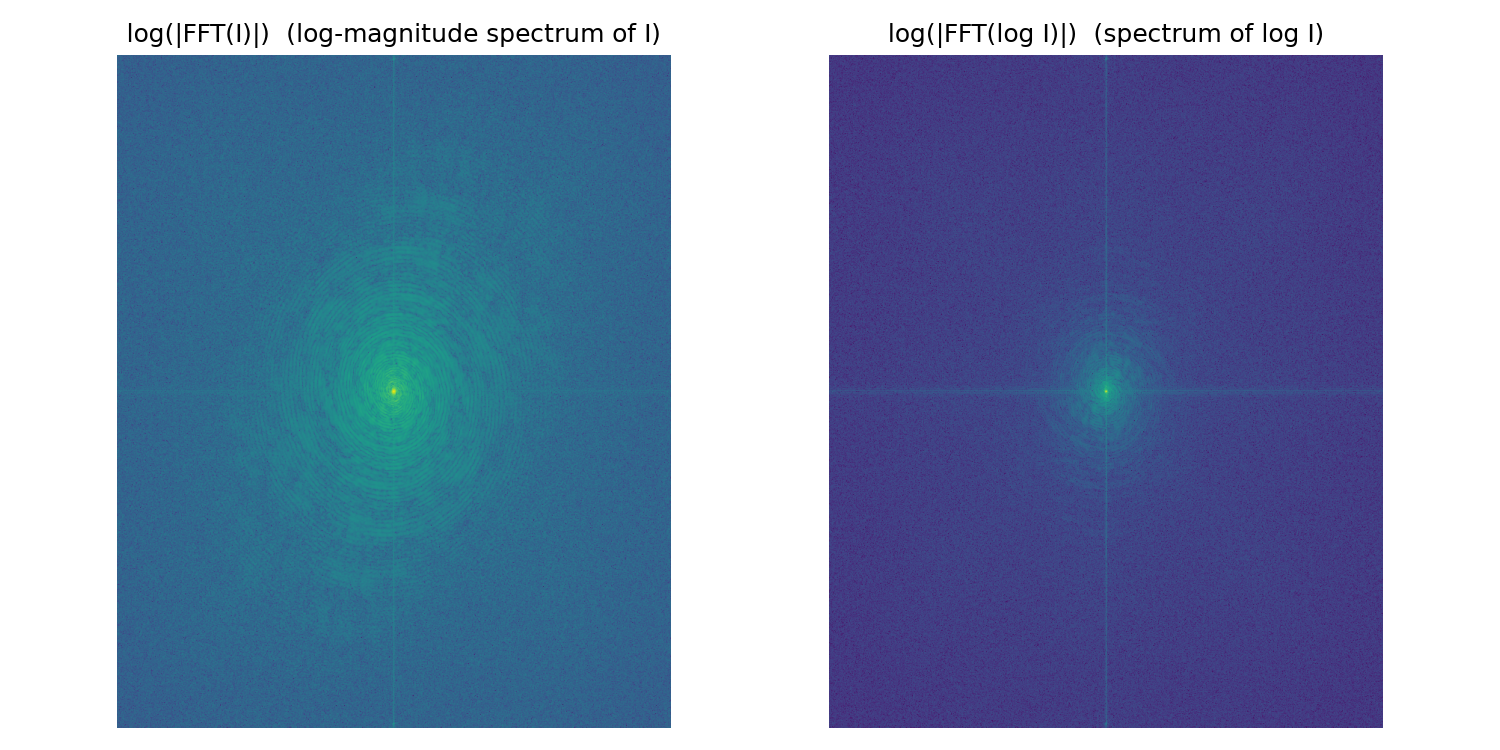
\includegraphics[width=0.8\linewidth]{results/3_1_log_order_demo.png}
  \caption{$\log|\mathcal{F}\{I\}|$ (left, the ordinary display log-magnitude spectrum)
  versus $\log|\mathcal{F}\{\log I\}|$ (right, the spectrum of the \emph{logged} image).
  The two are visually similar in coarse shape but are confirmed numerically distinct
  (correlation $0.669$ after normalisation), demonstrating that filtering one is not a
  substitute for filtering the other.}
  \label{fig:logorder}
\end{figure}

\subsection{Parameter sweeps}

\begin{figure}[H]
  \centering
  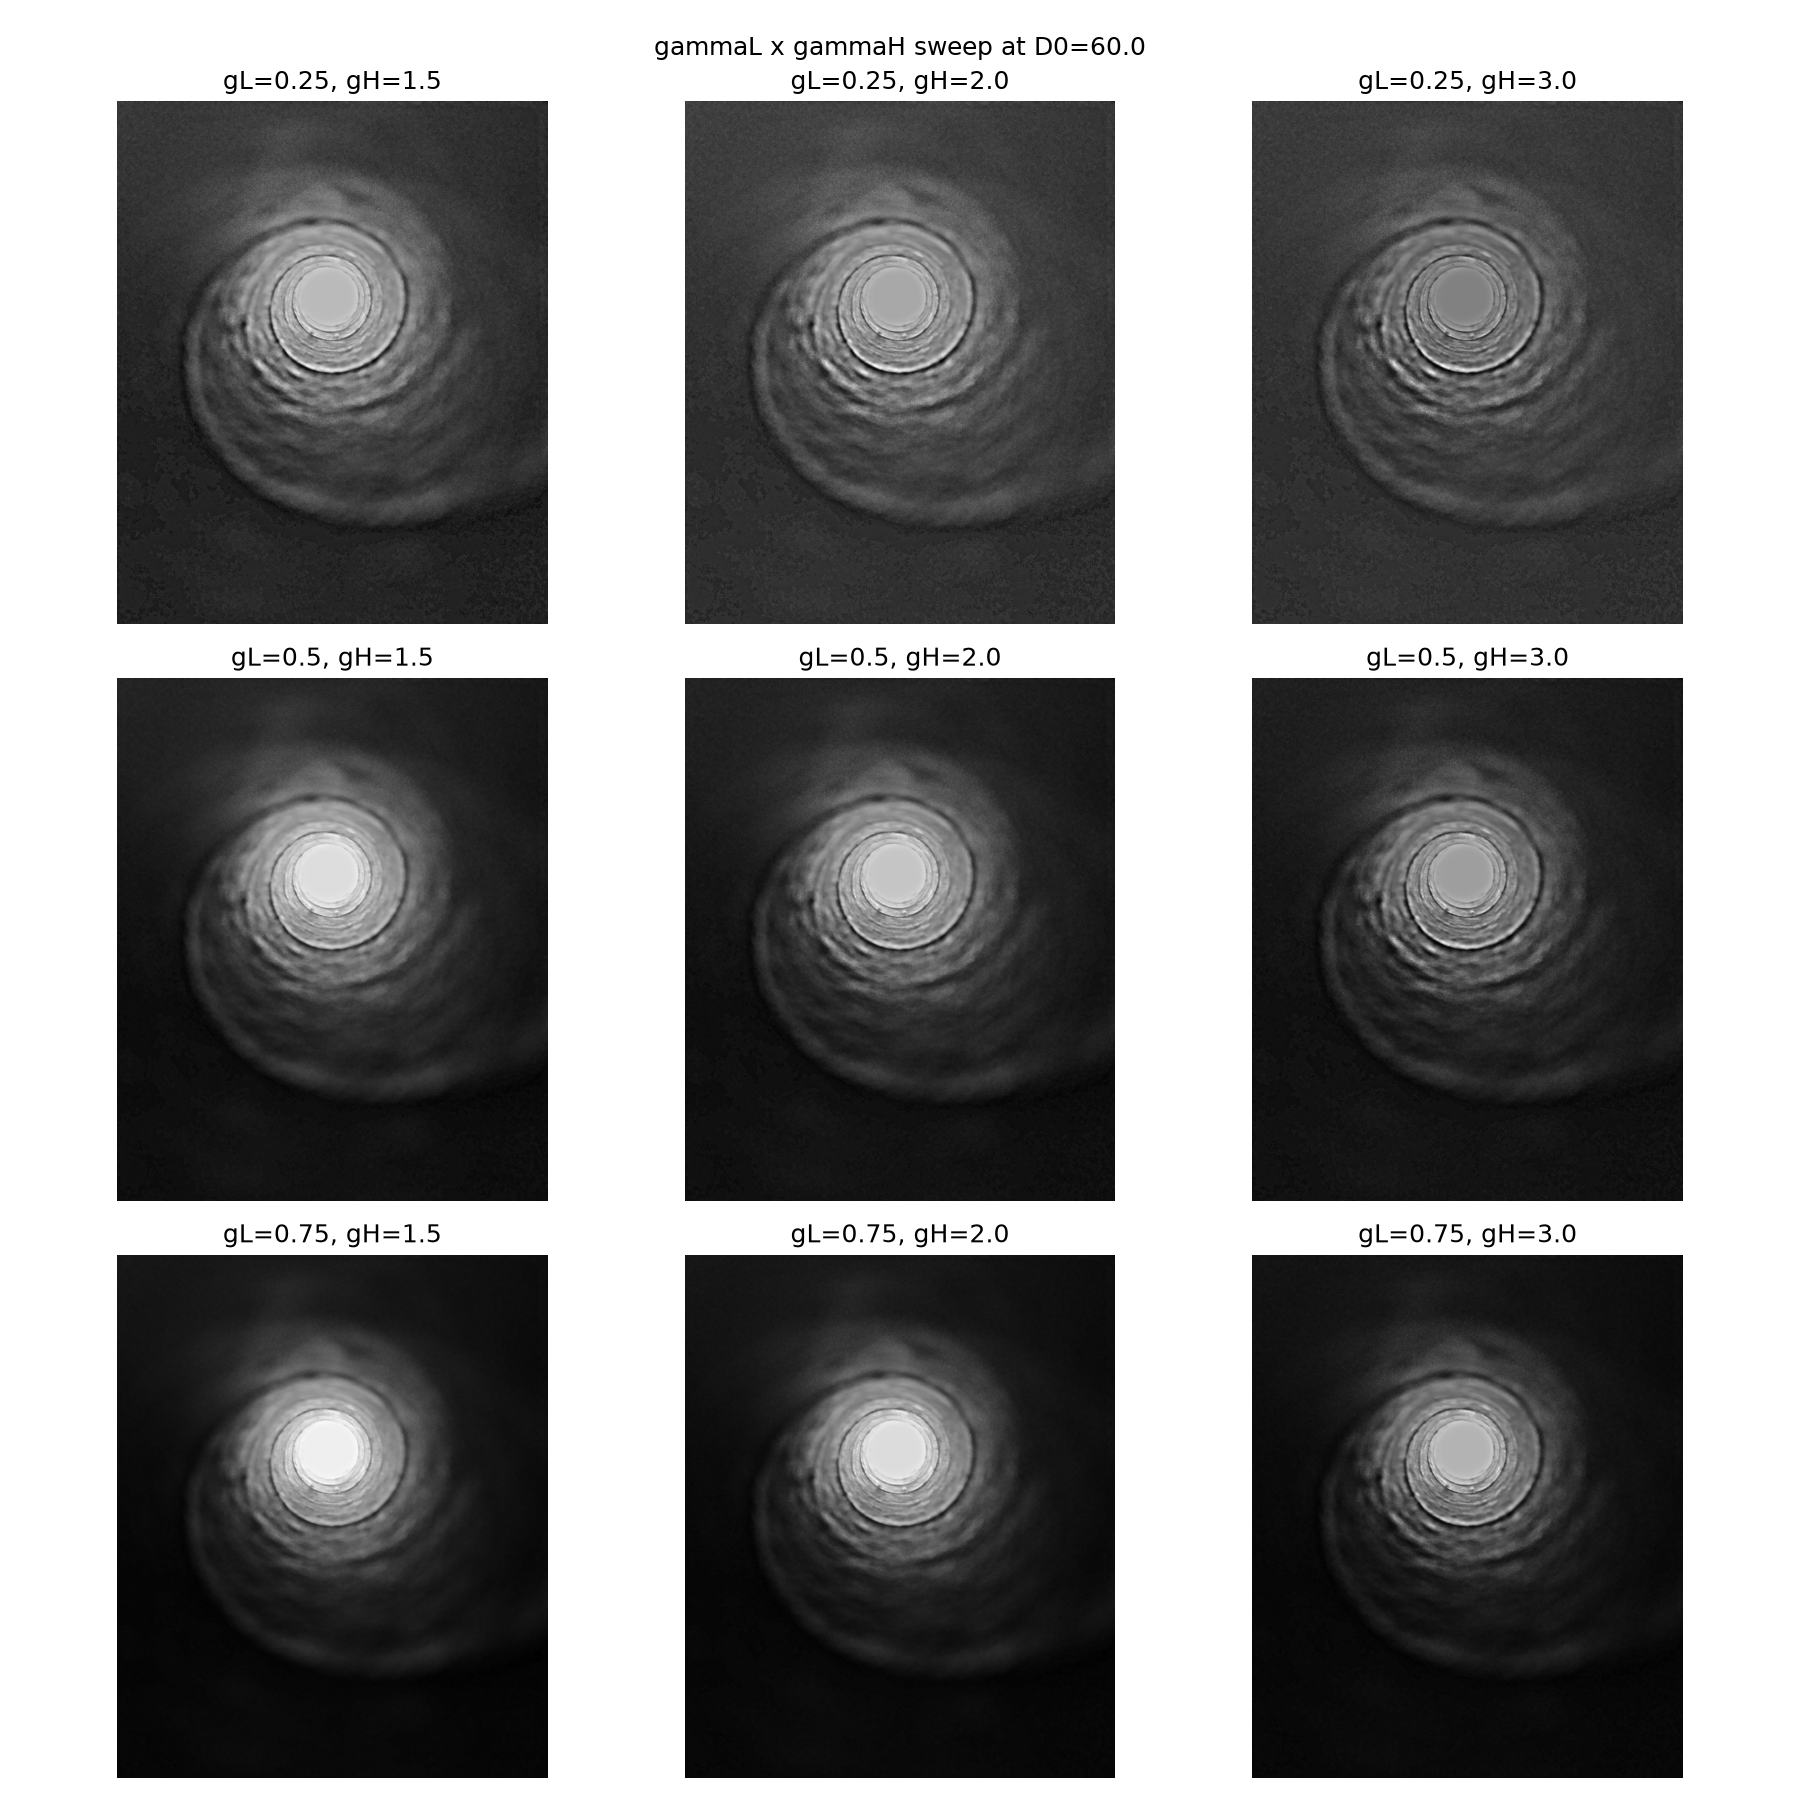
\includegraphics[width=0.8\linewidth]{results/3_2_gamma_sweep.png}
  \caption{$\gamma_L\in\{0.25,0.5,0.75\}$ (rows) $\times\ \gamma_H\in\{1.5,2.0,3.0\}$
  (columns) at fixed $D_0=60$. Lower $\gamma_L$ (top row) flattens illumination most
  effectively -- the tunnel wall's ring texture becomes visible almost uniformly across
  the whole frame, including what was deep shadow -- while higher $\gamma_L$ (bottom row)
  preserves more of the original illumination gradient, since a $\gamma_L$ close to 1
  barely attenuates the low-frequency illumination term at all. $\gamma_H$ mainly
  controls local contrast/sharpness of the recovered texture.}
  \label{fig:gammasweep}
\end{figure}

\begin{figure}[H]
  \centering
  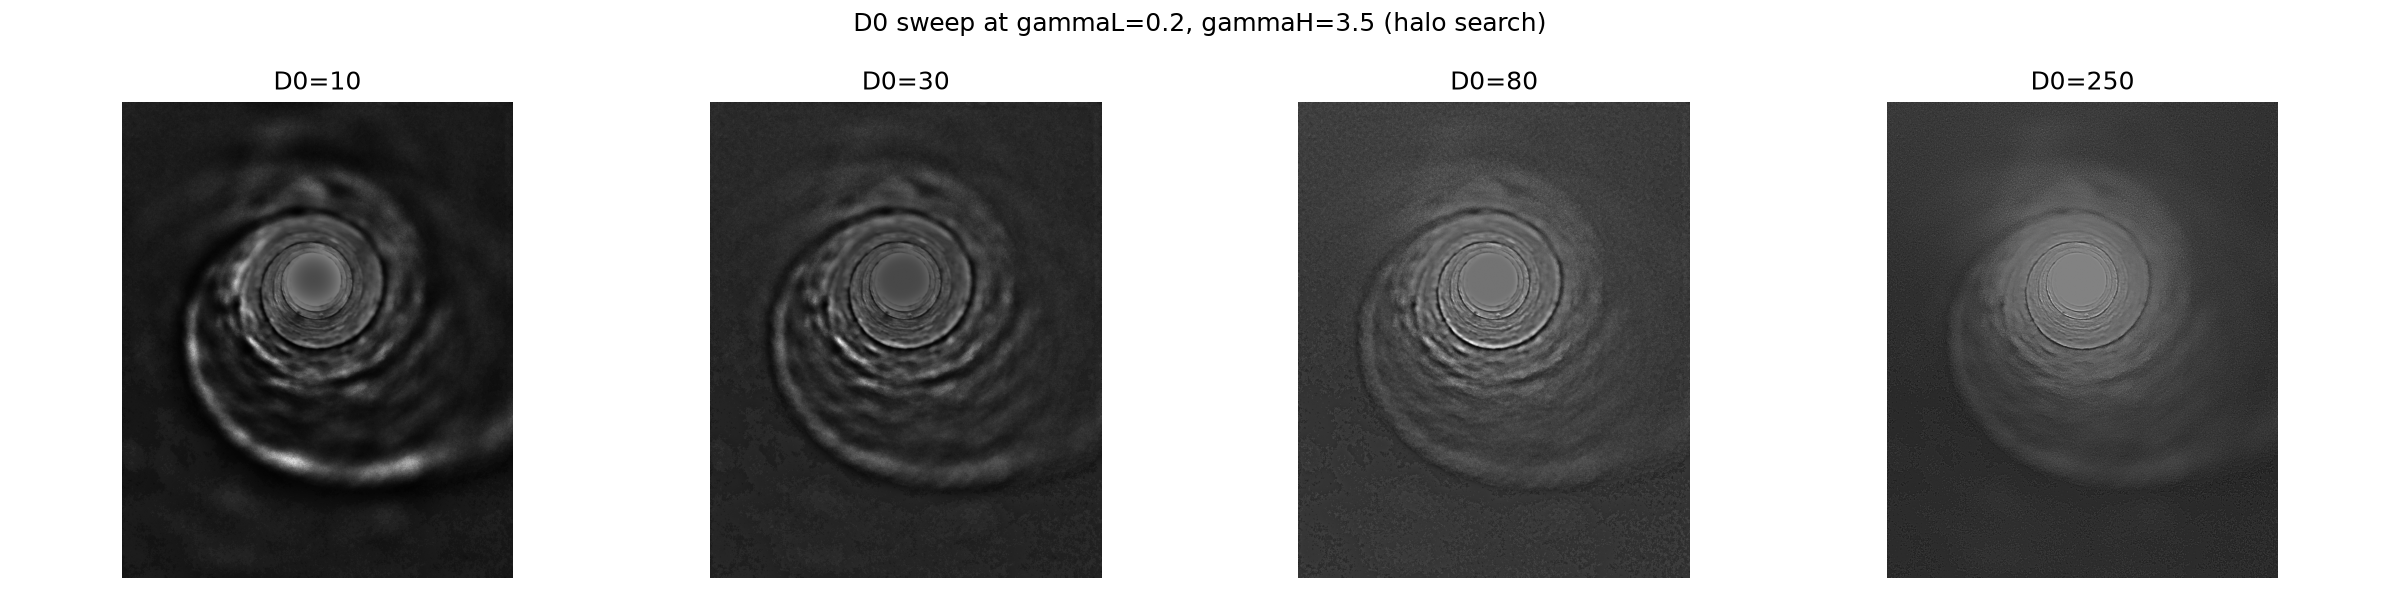
\includegraphics[width=0.8\linewidth]{results/3_2_D0_sweep_halo.png}
  \caption{$D_0\in\{10,30,80,250\}$ at a deliberately aggressive
  $\gamma_L=0.2,\gamma_H=3.5$. At $D_0=10$, a clear halo is visible: pronounced
  bright/dark ring-shaped banding around the light source and scalloped fringes through
  the wall texture, since the disc's edge sits right at the cutoff radius and the strong,
  broadband high-frequency gain rings around it. At $D_0=250$, the result is comparably
  smooth with no visible halo, but flattens illumination noticeably less well, since a
  larger $D_0$ classifies more of the genuinely slowly varying illumination as ``high
  frequency'' and leaves it comparatively un-boosted/un-flattened.}
  \label{fig:haloscan}
\end{figure}

\subsection{Best-tuned comparison against histogram equalisation}

\begin{figure}[H]
  \centering
  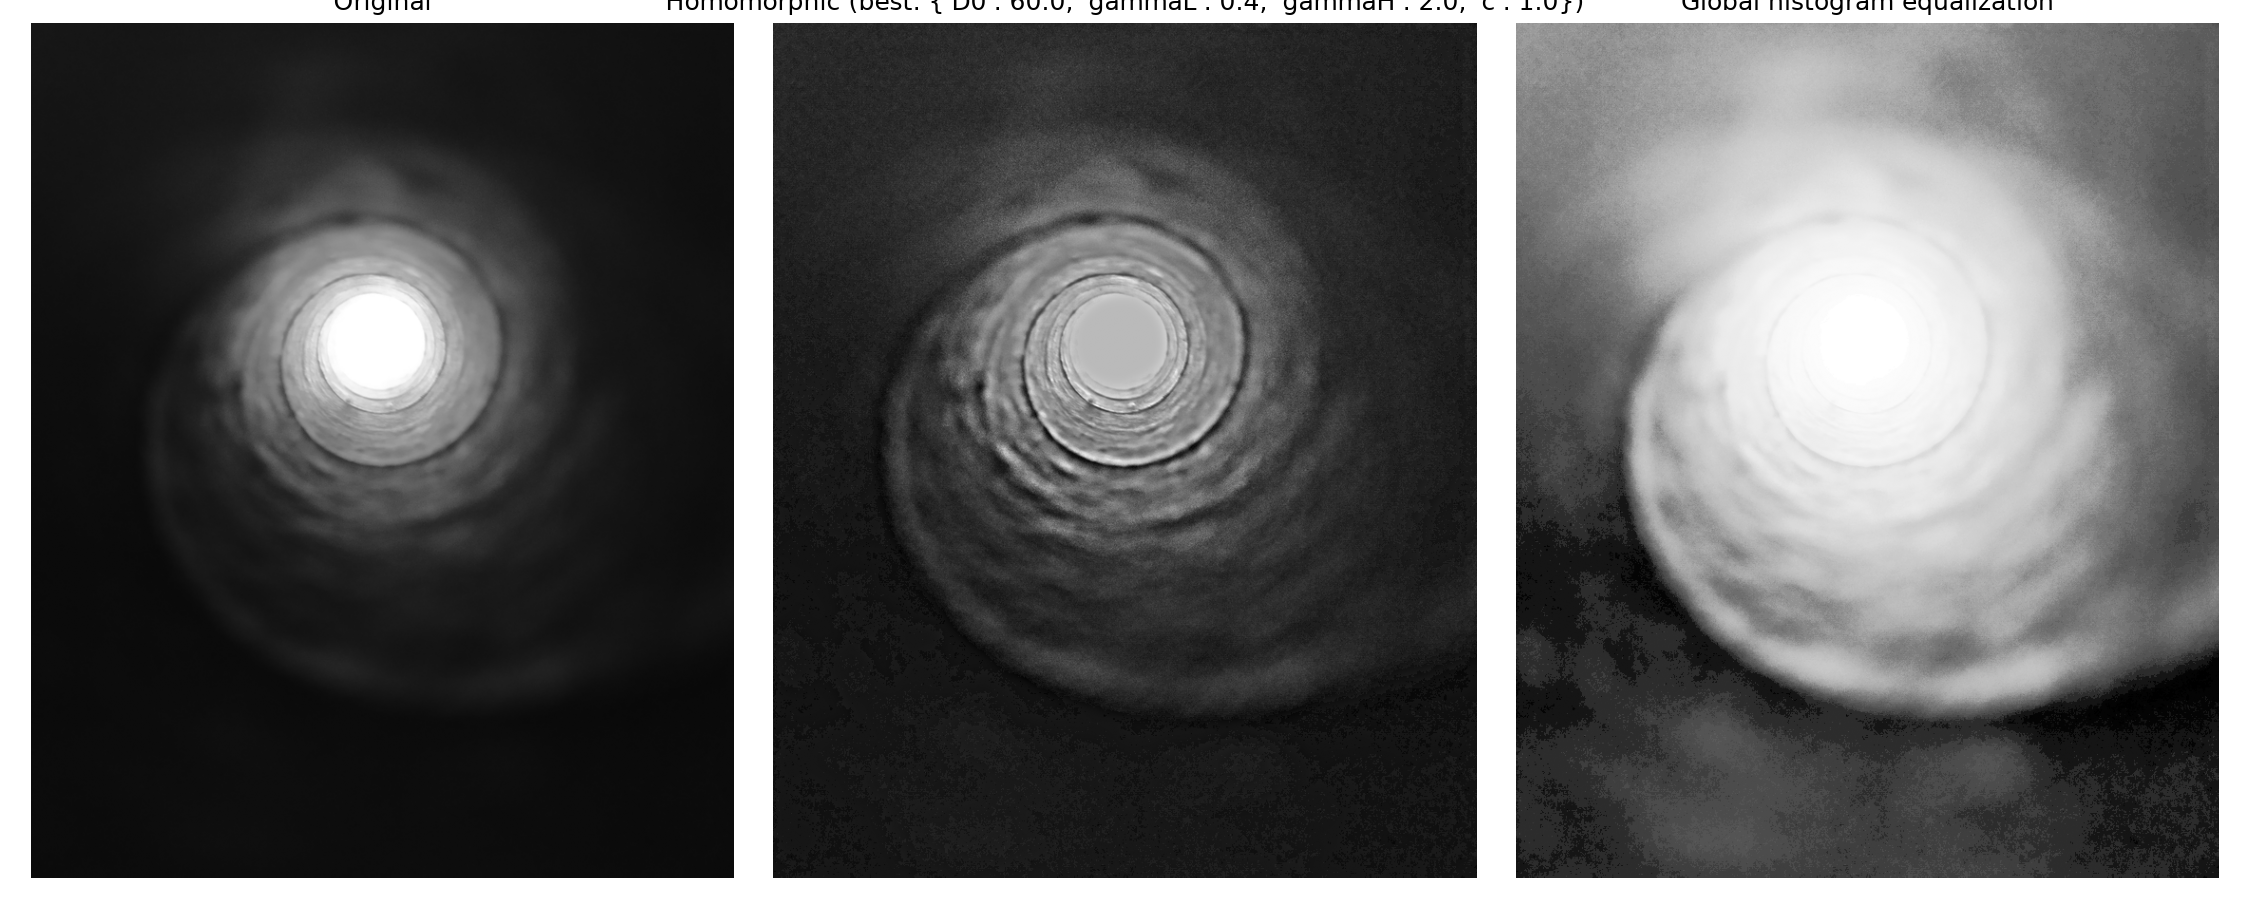
\includegraphics[width=0.8\linewidth]{results/3_2_comparison.png}
  \caption{Left to right: original image; best-tuned homomorphic output
  ($D_0=60,\gamma_L=0.4,\gamma_H=2.0,c=1.0$); global histogram equalisation. The
  homomorphic result visibly recovers wall-texture detail from the deep shadow while the
  light source is pulled back from saturation; histogram equalisation instead redistributes
  the whole image's histogram globally, amplifying shadow-region noise and leaving the
  bright region still saturated.}
  \label{fig:comparison}
\end{figure}

Table~\ref{tab:localcontrast} reports the data-driven local-contrast comparison, using a
$50\times 50$-pixel shadow block and bright block (identified automatically as the
darkest/brightest interior tile of the original image).

\begin{table}[H]
  \centering
  \caption{Local-contrast comparison between the original image, the best-tuned
  homomorphic result, and global histogram equalisation (exact figures from
  \texttt{results/3\_2\_result.json}).}
  \label{tab:localcontrast}
  \begin{tabular}{llrrr}
    \toprule
    Region & Metric & Original & Homomorphic (best) & Histogram eq.\\
    \midrule
    Shadow & mean & 10.41 & \textbf{17.68} & 12.82 \\
    Shadow & std (local contrast) & 0.86 & \textbf{5.38} & 14.72 \\
    Bright & mean & 255.00 & \textbf{185.76} & 254.999 \\
    Bright & max & 255.0 & \textbf{199.52} & 255.0 \\
    Bright & fraction $\ge 250$ & 0.9996 & \textbf{0.0} & 1.0 \\
    \bottomrule
  \end{tabular}
\end{table}

\textbf{Homomorphic filtering recovers shadow detail without blowing out the bright
region, clearly better than histogram equalisation here.} The shadow block's local
standard deviation (a direct proxy for local contrast) rises from $0.86$ (original,
essentially flat / noise-floor only) to $5.38$ under homomorphic filtering: real texture
has been pulled out of what was a nearly uniform black patch. Histogram equalisation's
shadow standard deviation (14.72) is numerically larger but for the wrong reason: global
histogram equalisation has no notion of \emph{where} in the image a pixel is, so it
simply redistributes the whole image's intensity histogram; because this image's
histogram is extremely imbalanced (dominated by near-black pixels), equalisation maps a
huge range of nearly indistinguishable dark values across a wide output range,
amplifying quantisation/compression noise in the shadow at least as much as genuine
structure, rather than the smooth, texture-revealing recovery that homomorphic filtering
achieves via the explicit illumination/reflectance model. More decisively, in the
\emph{bright} region, histogram equalisation still saturates $99.96\%\to100\%$ of pixels
at or above 250 -- it cannot do otherwise, since a monotonic global remapping preserves
rank order, so the brightest pixels in the original stay the brightest after equalisation,
pinned near 255 -- while the homomorphic filter's explicit illumination/reflectance
separation pulls the bright region's mean down to $185.76$ with \emph{zero} pixels left
at or above $250$, recovering structure in the light source too, not just the shadow,
which histogram equalisation cannot do by construction.

\section{Conclusion}

This problem demonstrated, both analytically and empirically, why a multiplicative
illumination--reflectance model requires a logarithmic transform \emph{before} any
linear frequency-domain operation can meaningfully separate its two components: the
log converts a product into a sum, and only sums can be split by frequency content
under a linear filter. The homomorphic high-frequency-emphasis filter of
Eq.~\eqref{eq:homfilter} was implemented and tuned on a strongly, unevenly lit tunnel
photograph, with $\gamma_L$ governing illumination suppression, $\gamma_H$ governing
reflectance/contrast boosting, and $D_0$ governing the trade-off between flattening
strength and halo risk. A real implementation pitfall was encountered and fixed along
the way: zero-padding, correct for the ordinary low-/high-pass filters of Problem 2,
produces a severe boundary ringing artefact under homomorphic filtering's strong
high-frequency gain, and was replaced with symmetric reflection padding. Quantitatively,
the best-tuned homomorphic result raised the shadow region's local contrast (std) by
over $6\times$ while fully eliminating bright-region saturation, outperforming global
histogram equalisation, which cannot distinguish illumination from reflectance and
therefore saturates the bright region regardless of how it redistributes the rest of
the histogram.

\end{document}
